\documentclass{article}

\usepackage{textcomp}
\usepackage{tikz}
\usepackage{amsmath}
\usepackage[hyphens]{url}
\usepackage{hyperref}
\usepackage[utf8]{inputenc}
\usepackage{relsize}
\usepackage{ifthen}
\usepackage{xstring}
\usepackage{cite}
\usepackage{placeins}

\newcommand{\crel}{
	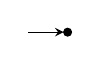
\begin{tikzpicture}[baseline={([yshift=-.8ex]current bounding box.center)}]
		\draw [->, >=stealth] (0,0) -- (0.45,0); 
		\draw [fill] (0.5,0) circle (0.05);
	\end{tikzpicture}
}

\newcommand{\rrel}{
	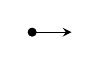
\begin{tikzpicture}[baseline={([yshift=-.8ex]current bounding box.center)}]
		\draw [fill] (0,0) circle (0.05);
		\draw [->, >=stealth] (0.05,0) -- (0.5,0);
	\end{tikzpicture}
}

\newcommand{\mrel}{
	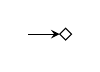
\begin{tikzpicture}[baseline={([yshift=-.8ex]current bounding box.center)}]
		\draw [->, >=stealth] (0,0) -- (0.4,0);
		\draw (0.4,0) -- (0.475,0.075) -- (0.55,0) -- (0.475,-0.075) -- cycle;
	\end{tikzpicture}
}

\newcommand{\irel}{
	\begin{tikzpicture}[baseline={([yshift=-.8ex]current bounding box.center)}]
		\draw [->, >=stealth] (0,0) -- (0.4,0);
		\draw (0.41,0) -- (0.55,0);
		\draw (0.48,-0.07) -- (0.48, 0.07); 
	\end{tikzpicture}
}

\newcommand{\erel}{
	\begin{tikzpicture}[baseline={([yshift=-.8ex]current bounding box.center)}]
		\draw [->, >=stealth] (0,0) -- (0.4,0);
		\draw (0.41,0) -- (0.55,0);
		\draw (0.48, 0.05) circle (0.02);
		\draw (0.48, -0.05) circle (0.02); 
	\end{tikzpicture}
}


\title{DCR/TEE \\
\large Working subtitle in a trusted execution environment}
\author{Mikkel Gaub \and Malthe Ettrup Kirkbro \and Mads Frederik Madsen}

% Allow line break at ',' in math mode:
\makeatletter
\def\old@comma{,}
\catcode`\,=13
\def,{%
  \ifmmode%
    \old@comma\discretionary{}{}{}%
  \else%
    \old@comma%
  \fi%
}
\makeatother

% C++ command
\newcommand\cpp{C\nolinebreak[4]\hspace{-.05em}\raisebox{.4ex}{\relsize{-1}{\textbf{++}}}}

\begin{document}
\sloppy

\begin{titlepage}
	\maketitle
	\pagenumbering{gobble}

	\vspace{\fill}
	\begin{abstract}
		In this thesis the security and optimization options provided by recent advances in trusted execution environments (TEE), specifically Intel Secure Guard Extensions (SGX), are explored in relation to the problem of decentralized partial state replication.
		An algorithm, and the implementation of that algorithm, for running decentralized Dynamic Condition Response (DCR) graphs is used as the example of a system requiring decentralized replication.
		Lastly a description of what it would require to transform the developed system to be able to handle general smart contracts is given.
	\end{abstract}
\end{titlepage}

\clearpage
\pagenumbering{arabic}

\tableofcontents

\newpage

\section{Introduction}

	In a time where collaboration between companies, small and large, occurs daily across vast physical distances, a trusted means of coordination is key.
	An example of this are Dynamic Condition Response (DCR) graphs, which is a declarative workflow management system.
	DCR graphs formulate processes in terms of events and relations between those events.
	The relations specify the order in which events can transpire, and what paths can be taken in the workflow.
	DCR graphs provide a concise and simple way of describing workflows, as executing an event can only affect events within a limited range, graph-wise.
	This means that DCR graphs allow for highly localized states and depending on how a specific DCR graph is constructed, it can therefore allow for a very high degree of concurrency.
	Central servers would be an easy solution to this problem, it would, however, require trust and payment, due to a third party being involved and managing the process.
	An alternative to central servers is, of course, a decentralized solution, with participants acting as peers in a peer-to-peer network. 
	This brings with it a completely different set of challenges, in that a core necessity of DCR is the agreement of all parties on what has transpired in the workflow and what the state of the workflow is at any given point, a non-trivial problem in decentralized DCR.
	
	As DCR graphs are concerned with maintaining a consistent state, the issue of making DCR graphs distributed is closely related to that of synchronizing distributed state replications.
	However, the innate properties of DCR graphs would be heavily constrained by existing solutions to distributed state replication, due to the large number of messages required and the low degree of concurrency provided by the strict synchronization of these algorithms.
	
	The problem, and solution, described in this thesis is not limited to applications of DCR, but can also be applied in other software concerned with maintaining a distributed, fragmented state.
	An example of such an application is also given, in the form of a distributed smart contract algorithm, as popularized by Ethereum \cite{_ethereum_2018}.
	The tools afforded to us by recent technological advances, provide strong guarantees and advantages which have already made waves within state replication solutions and which could potentially be leveraged to provide a solution to the described problem, while achieving the goals of a low number of messages and a high degree of concurrency.
	One such recent technological advancement are Trusted execution environments, such as Intel Software Guard Extensions (SGX), which provide a verifiable trusted subsystem to each participant, which is especially interesting in a decentralized system of mutually untrusting nodes.

	\noindent The contributions of this thesis are as follows:
	\begin{itemize}
		\item The design and implementation of a highly concurrent and fast distributed DCR engine, using SGX.
		\item A description of a generalized version of that design and implementation supporting arbitrary smart contracts rather than DCR graphs.
		\item A highly scalable algorithm for achieving consensus in a decentralized and distributed state replication system.
		\item An argument for the introduction of trusted execution environments reducing byzantine faults to crashes, in any distributed system.
	\end{itemize}

	\subsection{Problem}

	The goal is a decentralized DCR engine distributed among a number of actors, which allows for a graph to be distributed to and interacted with by each actor, in accordance with the specifications of the graph.
	Distributing DCR graphs is not a trivial problem, as there are considerations for the distribution of that graph, especially given the desire for a higher degree of concurrency than simply having all peers be responsible for the entire DCR graph.
	Alternatively, the DCR graph would have to be distributed on an event basis, but this is a much harder problem as changes only have to be propagated to the relevant events, meaning that multiple, possible conflicting, executions can happen simultaneously and would need synchronization intermittently.
	Actors interacting with the graph simultaneously should be allowed only when the ordering of those interactions is inconsequential.
	
	At any given time an actor should be able to collect the state of the graph and be ensured that any future state will not be incompatible with a previously collected state, with regards to the semantics specified by the graph.
	As DCR graphs provide rights on an actor to actor basis, it is unintuitive for the distribution of DCR graphs to support dynamic joining of the network and that is therefore not a requirement for a solution.

	In summary, the system must:
	\begin{itemize}
		\item Support the replication of a decentralized DCR graph, while maintaining a high degree of concurrency as permitted by the specific DCR graph.
		\item Achieve consensus on a state of a decentralized DCR graph in a number of messages by a factor of less than the number of nodes in the graph.
		\item Function in a highly malicious environment, where the only guarantees are those based on strong cryptographic security.
	\end{itemize}	

	\subsection{Related works}

	An existing platform which partially provides a solution to the goal of this project is Ethereum~\cite{_ethereum_2018}.
	Ethereum is a distributed computing platform based on blockchain technologies, which does, however, also feature a currency, making computations disproportionately expensive, both monetarily and computationally due to the large amounts of computations required by proof-of-work based blockchains.
	Even though SGX is a new technology, it has already been proposed to solve several issues in the blockchain concept. 
	SGX has been used as an intermediate for faster consensus about transactions in~\cite{gopinath_nirmala_improving_2017}, however it still relies on the underlying blockchain to prevent double-spending.

	In~\cite{liu_scalable_2016} SGX has been utilized to implement a new Byzantine fault tolerance (BFT) consensus algorithm, called \textit{FastBFT}, which solves some of the scalability issues of blockchains.
	This is done by using the \textit{strawman design} where a request is sent to a node, the \textit{primary}, who prepares a vote by distributing parts of a secret to all nodes.
	The secret can be reconstructed given enough parts and then compared to the hash of the secret which is common knowledge.
	This means that consensus can be achieved in only $O(n)$ messages, rather than the $O(n^2)$ messages achieved by other algorithms.
	The reason that Intel SGX is needed for this algorithm is that the primary, who distributes the secrets, can fake being any node as he has all parts of the secret.
	Trusted Execution Environments (TEE) as introduced by Intel SGX, means that these secrets can be computed and distributed without the primary every having access to them.
	A further issue with the strawman design, is that the primary can change the orders of requests, thereby equivocate which request is being voted on.
	This is once again solved by Intel SGX, by numbering requests with a trusted counter that can only be incremented.

	In particular, the Hyperledger Sawtooth~\cite{dhillon_hyperledger_2017} project is interesting as it is closely related to the goals of our project.
	Hyperledger Sawtooth is an ongoing blockchain project, which replaces the need for mining by using a consensus algorithm called Proof of Elapsed Time (PoET).
	In PoET a number of nodes who choose to participate as validators each create a timer using Intel SGX.
	This timer is different per validator and contains a timestamp some time in the future, with a degree of randomness.
	A validator can also check that a timer is valid, using Intel SGX, and also whether or not that timer has expired.
	The first validator to distribute a valid and expired timer to the rest of the validators, is elected leader for the current round of decision-making.	
	This is a strong indicator that Intel SGX can be used for efficiently attaining consensus.

\section{Background}

% Description of components covered in this section and why they are needed.

	\subsection{DCR}
	A DCR graph, $G$, is a graph representation of a workflow, made up of $v$ nodes, $E=\{e_1, e_2, \dots, e_v\}, v \geq 1$,  called \textit{events}, with a number of edges called \textit{relations} between them.
	Sometimes an event, $e$, in a graph, $G$, can be \textit{executed}, which will change the state and ability to execute of some events in $G$ according to the rules defined by $e$'s outgoing relations.
	We denote this execution $E(G,e)=G'$.

			\subsubsection{Event State}
			The events in a DCR graph have three binary attributes: \textit{included}, \textit{executed} and \textit{pending}. 
			This is an event: \ev{A}

			\begin{description}
				\item[Executed attribute] If an events \textit{executed} attribute is false executing the event will set its \textit{executed} attribute to true.
				Executing an already executed event will have no effect on the \textit{executed} attribute.
				The \textit{executed} attribute is shown as a tick mark: \ev[101]{A}
				\item[Pending attribute] If any event in a workflow has a \textit{pending} attribute that is true and the event is included, the workflow is in an unfinished state.
				Every time an event is executed its \textit{pending} attribute is set to false.
				This means that setting the \textit{pending} attribute of an included event to true is specifying that this event must be executed or excluded at some point to leave the workflow in a finished state.
				The \textit{pending} attribute is shown as an exclamation point: \ev[011]{A}
				\item[Included attribute] If the \textit{include} attribute of an event is false, the event is said to be excluded and it can not be executed.
				The \textit{included} attribute is denoted by the outline of the event: \ev{A} when included and \ev[000]{A} when excluded.
			\end{description}

			\subsubsection{Relations}
			\label{subsubsec:relations}
			There are five types of relations which define different types of relationships between events in a workflow.
			The origin and the target of a relation can be the same event.
			The five can be divided into two categories:

			\begin{description}
				\item[Effects] are relations that change the state of the targeted event. 
				If an effect originating from an event, \texttt{A}, is targeting an event, \texttt{B}, then \texttt{A} is said to be the effecting event on the effected event \texttt{B}.
				Effects are the \emph{response}, \emph{include} and \emph{exclude} relations. 
				\begin{description}
					\item[Response relation] If there is a response relation from event \texttt{A} to event \texttt{B}, then the \textit{pending} attribute of \texttt{B} will be set to true every time \texttt{A} is executed.
				The response relation is represented as: $\ev{A} \rrel \ev{B}$
					\item[Include relation] If there is an include relation from event \texttt{A} to event \texttt{B}, then the \textit{included} attribute of \texttt{B} will be set to true every time \texttt{A} is executed.
				The include relation is represented as: $\ev{A} \irel \ev{B}$
					\item[Exclude relation] If there is an exclude relation from event \texttt{A} to event \texttt{B}, then the \textit{included} attribute of \texttt{B} will be set to false every time \texttt{A} is executed.
				The exclude relation is represented as: $\ev{A} \erel \ev{B}$
				\end{description}
				\item[Constraint] are relations that exclusively affect whether or not the targeted event can be executed. 
				If a constraint originating from an event, \texttt{A}, is targeting an event, \texttt{B}, then \texttt{A} is said to be the constraining event on the constrained event \texttt{B}.
				Constraints are the \emph{condition} and \emph{milestone} relations. 
				\begin{description}
					\item[Condition relation] If there is a condition relation from event \texttt{A} to event \texttt{B}, then \texttt{B} can only be executed if the \textit{executed} attribute of \texttt{A} is true or the \textit{included} attribute of \texttt{A} is false.
				The condition relation is represented as: $\ev{A} \crel \ev{B}$
					\item[Milestone relation] If there is a milestone relation from event \texttt{A} to event \texttt{B}, then \texttt{B} can only be executed if the \textit{pending} attribute of \texttt{A} is false or the \textit{included} attribute of \texttt{A} is false.
				The milestone relation is represented as: $\ev{A} \mrel \ev{B}$
				\end{description}
			\end{description}

			\subsubsection{Enabledness}
			Since the properties of DCR graphs described so far all affect whether or not a given event can be executed or not, we use the notion of enabledness to describe the sum of these properties.
			An event which can be executed, meaning it is included and any milestones or conditions targeting it are rendered invalid by the state of the relevant events, it is said to be enabled.
			If an event cannot be executed, due to the inverse of the aforementioned prerequisites, it is said to be disabled.
			If an event changes from being enabled to disabled or from disabled to enabled, its enabledness is said to have changed.
			Formally, we say that $E(G,e_1) = G$ if $e$ is not enabled.

			\subsubsection{Formalising \texorpdfstring{$G$}{}}
			After the previous definitions, we can now formalise the concept of a DCR graph $G$:
			$G = (E, I, P, Ex, En, R)$, where
			\begin{itemize}
				\item $E$ is the set of all events.
				\item $I \subseteq E$ is set of the included events.
				\item $P \subseteq E$ is the set of pending events.
				\item $Ex \subseteq E$ is the set of excluded event.
				\item $En \subseteq E$ is the set of enabled events.
				\item $R = \{r_1, r_2, \dots r_e\}$ is the set of relations, where each relation, $r$, has the form $r=(e_{from}, e_{to}, Type)$ and $e_{from}$ is the event for which $r$ is directed from, $e_{to}$ is the event for which $r$ is directed to, and $Type$ is one of the relation typed described in section~\ref{subsubsec:relations}.
			\end{itemize}

			\subsubsection{Concurrency}
			The notion of concurrency in DCR graphs, described in~\cite{debois_concurrency_2015}, is the property a pair of events is said to have when the graph allows those events to be executed in either order with the same resulting state in graph.

			More formally, given a graph, $G$, and two events $e_1, e_2$ in $G$, we say that $e_1$ and $e_2$ are concurrent if $E(E(G, e_1),e_2)=E(E(G, e_2),e_1)$.

			If two events are concurrent, we say that they are independent.
			There are two types of independence analyses relevant for this paper:
			\begin{description}
				\item[Dynamic independence] means that for two given events and their current state, are they independent.
				That is, $e_1$ and $e_2$ are dynamically independent if $E(E(G, e_1),e_2)=E(E(G, e_2),e_1)$ for the current $G$.

				We say that an event, $e$, has a \textit{dynamic independence set}, $I_{dyn}(G,e)$, such that $e' \in I_{dyn}(G,e)$ iff. $e$ and $e'$ are dynamically independent in graph state $G$.
				Likewise an event, $e$, has a \textit{dynamic dependence set}, $D_{dyn}(G,e) = E \setminus I_{dyn}(G,e)$.
				\item[Static independence] means that two events, are dynamically independent in every \textit{reachable} state of the graph, where they are both enabled.
				That is, $e_1$ and $e_2$ are statically independent in $G$, if they are dynamically independent in all states of $G$ that can be reached by a sequence of event executions.

				We say that an event, $e$, has a \textit{static independence set}, $I_{stat}(e)$, such that $e' \in I_{stat}(e)$ iff. $e$ and $e'$ are statically independent.
				Likewise an event, $e$, has a \textit{static dependence set}, $D_{stat}(e) = E \setminus I_{stat}(e)$.
				This problem is NP-hard and an approximation will have to be used instead~\cite{debois_concurrency_2015}.
			\end{description}

			The approximation we use of static event independence is from~\cite{debois_concurrency_2015}, and boils down to the following principles, where we say that $e_1$ and $e_2$ are approximately statically dependent if, in any event-state permutation of $G$: %forklar event-state permutation?
			\begin{itemize}
				\item $e_1$ can enable $e_2$, and vice versa.
				\item $e_1$ can disable $e_2$, and vice versa.
				\item $e_1$ can disable some $e$, if $e_2$ can enable it, and vice versa.
				\item $e_1$ can exclude some $e$, if $e_2$ can include it, and vice versa.
				\item $e_1$ can set $e_2$ to pending, unless $e_2$ sets itself to pending, and vice versa.
			\end{itemize}
			This approximation is sound, but incomplete, which means that it contains all statically dependent event pairs, but does not guarantee that an event pair in the approximation is not statically independent in the specific graph on which it is run.

			We say that an event, $e$, has an \textit{approximate static dependence set}, $D_{appr}(e)$, such that $e' \in D_{appr}(e)$ iff. $e$ and $e'$ are approximately statically dependent, according to the above approximation.
			Likewise an event, $e$, has an \textit{approximate static independence set}, $I_{appr}(e),  = E \setminus D_{appr}(e)$.

			Notice that all the independence- and dependence sets are reflexive: $e' \in S(e) \iff e \in S(e')$, where $S$ is any of the described (in-)dependency sets.

			Figure~\ref{fig:concurrency-all} shows examples of independence in DCR graphs.

		\begin{figure}[!ht]
			\center
			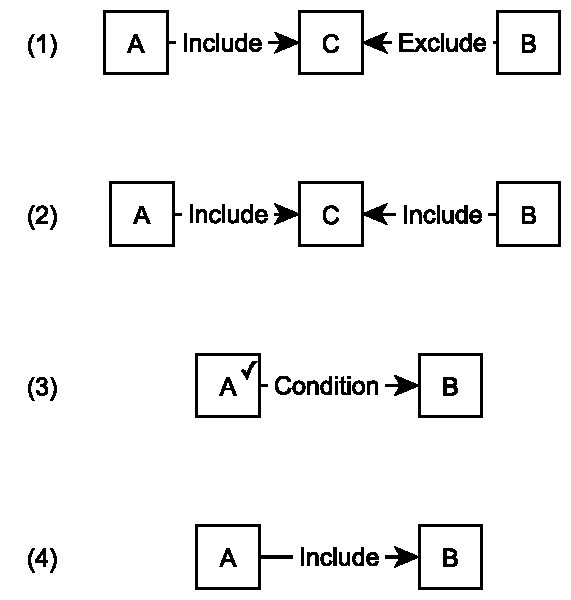
\includegraphics[scale=0.6]{figures/dcr-graphs/concurrency-all.pdf}
			\caption{From top to bottom:
			(1) An example of a DCR graph where \ev{A} and \ev{B} are not concurrent.
			(2) An example of a DCR graph where \ev{A} and \ev{B} are statically independent.
			(3) An example of a DCR graph where \ev{A} and \ev{B} are dynamically, but not statically independent.
			(4) An example of a DCR graph where \ev{A} and \ev{B} are statically independent, but the approximation will contain them as a dependent pair\label{fig:concurrency-all}.}
		\end{figure}

			% Independent exec: ændrer til det samme, eller ikke rører ved ? 
			% Independent enab: Læser ikke hvad du skriver ? 
			% Backwards og forwards validation ? 

			\subsubsection{Execution rights}
			For DCR graphs to have a meaningful application, each event is typically assigned a number of actors who are allowed to execute that event.
			Rights to execute can also be assigned based on role.



		\subsection{Consensus}
		Consensus is the problem of achieving agreement between the processes in a distributed system. 
		It is central to the the problem of distributed DCR, as agreement on the states of event must be achieved to ensure that all correct peers adhere to the semantics of the DCR graph. 
		Take the simple graph $\ev{A} \crel \ev{B}$, and let a subset of peers $p_1$ be responsible for the state of $\ev{A}$, and a subset of peer $p_2$ be responsible for the state of $\ev{B}$.
		If agreement on the state of $\ev{A}$ is not guaranteed, then $p_2$ might, in the belief that $\ev{A}$ is executed, execute $\ev{B}$ even though $p_1$ has never executed $\ev{A}$. 

		A consensus protocol is formally as a protocol with $N$ processes ($p_0, p_1, \dots, p_{N-1}$), where each process $p_i$ begins in an undecided state, and proposes a single value $v_i$ from a set of values $D$. The processes then communicate their values to each other, and each process sets a decision variable $d_i$ and enters a decided state. For the protocol to solve the consensus problem, the following requirements should hold for every execution:
		\begin{description}
			\item[Termination:] every process eventually sets its decision variable.
			\item[Agreement:] the decision variable of all correct processes are the same.
			\item[Validity:] if a correct process decides $d$, then some correct process has proposed a value $v$, where $v = d$.
		\end{description}

		It's easy to see that distributed DCR reduces to consensus.
		The reduction without any concurrency goes like this:\\
		\noindent
		We assume that the correct graph has been distributed to all peers, and initial state is agreed upon.
		\begin{itemize}
			\item Let $D$ be the set of enabled events.
			\item Let $v_i$ be an identifier an event. 
			\item A correct process will only propose $v_i$ if the event identified by $v_i$ is enabled.
			\item We can now use a consensus sub-process to decide on a $v$, which will then be executed.
			\item Each process recalculates $D$ to reflect the new global state, and repeats the protocol until the workflow has been completed.
		\end{itemize}

		In the famous FLP impossibility result from 1985~\cite{fischer_impossibility_1985}, it was shown that non-termination was possible in all consensus protocol systems with asynchronous communication channels and at least one (crash)faulty process.
		In order to circumvent this impossibility, the guarantees of a fault-tolerant system that utilizes a consensus protocol are relaxed, for instance by guaranteeing Termination only when no faults are present, as is the case in  the Paxos protocol~\cite{lamport_part-time_1998}. 

		\subsubsection{State Machine Replication}
		One problem that relates directly to consensus, is \textit{State Machine Replication} (SMR).
		SMR is the problem of replicating the state of a system on several nodes, called \textit{replicas}.
		Replicas are modelled as state machine.
		In SMR systems, \textit{clients} send requests to replicas who must then guarantee:
		\begin{description}
			\item[Safety:] all non-faulty replicas execute the requests in the same order.
			\item[Liveness:] clients eventually receive replies to their requests.
		\end{description}
		The state machine replication problem is equivalent to the consensus problem and essentially provides the same guarantees~\cite{schneider_implementing_1990}. 
		This is evident in the fact that the safety requirement is essentially an aggregation of the agreement and validity requirements in consensus, while the liveness property is equivalent to termination.  
		Equivalent to consensus. 
		As such, FLP impossibility entails that one of the requirements must be relaxed in fault tolerant SMR systems.
		This is often done by only guaranteeing liveness when no failures are present.

		A version of SMR deals with byzantine faults, instead of crash failures.
		These systems are knowns as \textit{byzantine fault tolerance} (BFT) systems.
		These systems deals with arbitrary faults, that is arbitrary behaviour of faulty processes and channels, including changing messages, creating new messages and changing local state. 
		It has been shown that $2f+1$ processes are necessary and sufficient to solve SMR with relaxed liveness if faulty processes only exhibit crashes~\cite{bracha_asynchronous_1985}. 
		Similarly it has been shown that $3f+1$ processes are necessary and sufficient to solve SMR with relaxed liveness if faulty processes can exhibit byzantine faults~\cite{bracha_asynchronous_1985,pease_reaching_1980}.
		Recent advances have been made in BFT-algorithms, which increase fault tolerance from $3f+1$ to $2f+1$ by utilizing TEE features~\cite{liu_scalable_2016,kapitza_cheapbft_2012,veronese_efficient_2013}.
		When we take the proofs of sufficient and necessary amounts of processes in BFT systems into account, these advanced strongly indicates that TEEs might be able to reduce byzantine faults to crash faults, a statement we will explore further in section \ref{sec:transforming-byzantine-faults}.
		SMR brings with it the taxing job of pushing each update to all nodes in the network, which leads to obvious scalability issues in large networks.

		One solution to that problem is delegating the responsibility of segments of data to each node in the network.
		This is called \textit{Partial State Machine Replication} (PSMR).
		PSMR, by necessity, allows multiple simultaneous leaders and only synchronizes state changes when those state changes are conflicting.
		Due to allowing multiple leaders, PSMR provides high availability as any node can request a state change.
		High concurrency and performance also follows from the partial states reducing the number of nodes which have to be notified of a state change leading to both fewer messages and less chance of two state changes overlapping, requiring ordering.
		Relatively few solutions exists for the PSMR problem and the ones that do require a large amount of messages \cite{sousa_partial_2001}.
		To the best of our knowledge, no solution to the PSMR problem using a trusted execution environment exists.

		\subsection{Intel SGX}

		Intel SGX is a TEE technology which allows users to define protected areas of memory, so called \textit{enclaves}.
		Intel guarantees~\cite{intel_sgx} that any code run and data loaded in the TEE is protected from access by any process running outside of the enclave.
		More specifically, the guarantees encompass \textit{confidentiality}, i.e. no other process can read the data in the enclave, and \textit{integrity}, i.e. no other process can modify the data in the enclave. 
		If the enclave contains secrets which the user wishes to keep, but still does not want to trust external processes with, the enclave can be sealed on disk, essentially encrypting it for later use.
		This means that data can be stored and processed securely, with its security guaranteed by Intel, if done properly.
		An additional feature of Intel SGX is that the result of any code run using Intel SGX can be verified by other users, given the code and the output.

		This is all made possible by unique keys generated during manufacturing and permanently stored inside the fuse array of the processor.
		Some of these keys are known by Intel for the system to be recognized when contacting Intel servers.

		In short, the major innovation in Intel SGX is the option of running hardware secured software, which enables tamper proof messages, where the sender can be verified as being a correct process.
		This eases some of the inherent problems in consensus, as seen in~\cite{liu_scalable_2016} and~\cite{dhillon_hyperledger_2017}.

			\subsubsection{Enclave}
			\label{subsec:enclave}
			What allows SGX enabled CPUs to provide these strong guarantees builds on the following two hardware details:
			\begin{description}
				\item [Processor Reserved Memory (PRM)] is a sequential block of memory reserved for SGX, inaccessible from untrusted software and even hardware.
				\item [Enclave mode] is a mode under which a logical processor gains access to the PRM.
			\end{description}
			Using these hardware facilities SGX defines the concept of an enclave.
			An enclave is, as its name suggests, a software module isolated completely from the rest of the system.
			Its memory is located solely in PRM, preventing access by other processes and enclaves running on the system. 
			The PRM is protected from non-enclave processes by enclave mode. 
			When a process is not in enclave mode and tries to access the PRM, the memory access is denied~\cite{costan_intel_2016}.      
			The PRM of an enclave process is protected from accesses by other processes in enclave mode by the SGX Enclave Control Structure (SECS). 
			The SECS holds meta data about the enclave processes, and among this is a virtual-to-physical memory mapping called the Enclave Page Cache (EPC). 
			Through the EPC an enclave's access to physical PRM is restricted to what has been allocated for the enclave-process~\cite{costan_intel_2016}.

			While SGX provides powerful guarantees trough its enclave concept, it does not guarantee software correctness and will not protect against flawed software.
			Instead SGX encourages developers to isolate a minimal piece of their software, the Trusted Computing Base (TCB), in a trusted enclave environment, and keep the remainder as traditional system processes~\cite{intel_sgx_guide}.
			By minimizing the size of the TCB, and thus the amount of code one must trust, common security principles indicate that the chance of security flaws decreases~\cite{intel_sgx_guide}.

			In order for an isolated enclave to be useful, communication between trusted and untrusted software is enabled through \textit{enclave calls} (ECALL) and \textit{out calls} (OCALL).
			This interface must be defined at compile-time, specifying an API of ECALLs for the enclave as well as any untrusted services needed as OCALLs, in a \textit{EDL}-file~\cite{intel_sgx_guide}.

			When built, an enclave module is a plain binary on the untrusted file system.
			As an enclave under such circumstances would be vulnerable to tampering before initialization, SGX enforces a strict signature policy.
			An enclave must include an \textit{Enclave Signature} containing \textbf{(a)} a hash of the code and initialization data of the enclave, \textbf{(b)} the author's public key and \textbf{(c)} an enclave version/product number.
			During enclave initialization a hardware check is performed, ensuring the Enclave Signature matches the enclave binary loaded from the file system.

			Another powerful tool of an SGX enclave is the ability to read from and write data to an untrusted storage medium while ensuring confidentiality of its contents.
			Such capabilities are needed as the PRM is volatile and will not persist after shutdown.
			In SGX this process is known as \textit{sealing}.
			Sealing allows encryption and decryption using a \textit{Seal Key}, which is confidential to the Enclave Signature.

			However, these mechanics alone does not guarantee integrity, as integrity is not only violated by other processes.
			For instance, the infamous Single Upset Event (also knowns as cosmic ray bit flips)~\cite{normand_single_1996}, is an integrity violation where bits in memory are flipped due to background radiation. 
			Intel SGX protects against such hardware errors by using cryptographic integrity checks~\cite{gueron_memory_2016}.
			When loading enclave memory, Intel SGX's Memory Encryption Engine (MEE) decrypts the memory, and then performs an integrity check on the loaded memory.
			If the integrity check does not pass, the processor drops the memory, and eventually locks itself for further operations (the \textit{drop-and-lock policy}), requiring a physical reset before new operations can be completed~\cite{jang_sgx-bomb_2017}.

			In short, the integrity checks is implemented as a Merkle-Tree of Message Authentication Codes (MACs), with the root node of the tree stored on processor-internal memory~\cite{jang_sgx-bomb_2017}. 
			Under the assumption that AES128 is a random permutation, this method provides the guarantee that an active adversary with the capability of observing the MACs has a negligible probability of forgery~\cite{gueron_memory_2016}.

			A practical example of the effectiveness of this integrity check is the \textit{SGX bomb} attack~\cite{jang_sgx-bomb_2017}. 
			The SGX bomb, is a denial-of-service attack on Intel SGX. 
			It utilises a Row hammer attack to flip arbitrary bits in the EPC, thus triggering the drop-and-lock policy when memory is loaded.

			\subsubsection{Attestation}
			\label{subsec:attestation}
			Attestation, within the Intel SGX platform, is the action of verifying the existence of specific enclaves.
			The applications of this are two-fold, in the case where there are multiple enclaves running locally on the same CPU and in the case where enclaves need to communicate to enclaves running on external CPUs.
			These two situations are handled by two different processes, aptly named local and remote attestation.
	  
			Local attestation builds on a secret fused into the CPU.
			An enclave can use an SGX instruction to generate a report uniquely identifying the enclave.
			This report is MACed with a key derived from the fused secret and enclave identifier.
			It is not possible to fake such a MACed report, as the MACing happens in hardware components that ensure that the report corresponds to the caller enclave.
			The fused secret is not directly accessible by software components, but can only be used by certain hardware instructions that protect against malicious use.
			An attestation challenger will ask for a MACed report from the client enclave, and after receiving it derive the same key to verify the MAC.
			Because a report can only be created by the enclave it describes, the challenger can be certain of which enclave the client is running if the MAC is valid.
			To prevent replays the MACed report is allowed to contain a block of arbitrary data, in which the challenger can require a nonce.

			Remote attestations build on the same concept of a report, but as challenger and client are now on different CPUs, they no longer hold the same fused secret.
			Instead remote attestation relies on the group signature scheme Enhanced Privacy ID (EPID) and a third party issuer.
			Each SGX enabled CPU is granted an EPID Member Private Key by the third party issuer some time after manufacturing.
			Like the fused secret, this private key is not directly accessible to an enclave.
			Under the EPID scheme, all issuer generated private keys share the same public key (EPID Group Public Key).
			When remote attestation takes place, the client enclave generates a report and attests locally with the Quoting Enclave (QE).
			The QE, now convinced of the client enclave's identify, strips the MAC off the report and instead signs it with the EPID Member Private Key, which the QE has special privileges to access\footnote{Enclaves signed by Intel have special privileges throughout SGX. This allows SGX to implement complicated SGX instructions in software.}.
			The remote challenger can verify the signed report with the EPID Group Public Key and be sure that \textbf{(a)} the report is signed by an EPID Member Private Key, \textbf{(b)} EPID Member Private Keys are granted secret to QEs, and \textbf{(c)} QEs will not sign false reports.

			%TODO, Mangler, sdf: Præcis beskrivelse af remote attestation process. 

			\subsubsection{Monotonic counters}
			One of the functions provided by Intel SGX, which is especially relevant for this project, is the access to \textit{trusted monotonic counters}.
			As indicated by the name, monotonic counters are integer counters, that can only be incremented.
			They are implemented as a block of non-volatile memory accessible only through SGX instructions, protecting against replay attacks.

	\section{System model}
	We consider a system of $n$ processes $P=\{p_1, p_2, \dots, p_n\}$, that communicate through message passing channels.
	The system is asynchronous, in the sense that we make no assumptions about the execution speed of processes, or delivery time of messages.

	We assume a byzantine fault model, in that processes may fail by exhibiting arbitrary behaviour, except for enclave components which can only exhibit crash-failures because of the integrity and confidentiality guarantees given by Intel SGX.
	We also assume that byzantine faults cannot corrupt data that has been cryptographically signed or encrypted by an enclave, in such a way that the data is still correctly signed/encrypted by the same key after the data has been corrupted. 
	Byzantine faults includes, but are not limited to, crashes and arbitrary change of local state.
	Processes that never fails are \textit{correct}, and processes that are not correct are \textit{faulty}.
	Notice that after section \ref{sec:transforming-byzantine-faults} we will only consider crash-faults, due to the argument that Intel SGX can, in a system where faulty processes can exhibit byzantine faults, make correct processes exhibit behaviour equivalent to the faulty processes being crashed.

	The system includes a DCR-graph, $G$, which consists of $v$ events $E = \{e_1, e_2, \dots, e_v\}$. %, such that $n > m$. %\geq 3m$??? 
	Each $p$ stores the state of a subset of the events, $E_p$, such that $E_{p_1} \cup E_{p_2} \cup \dots \cup E_{p_n} = E$.
	The number of $p$s that stores an $e$'s state is the \textit{replication factor} of $e$, denoted $\rho_e$.
	$E_{p_1} \cup E_{p_2} \cup \dots \cup E_{p_n} = E \implies \rho_e \geq 1$, for all $e$.
	Or in other words, each event's state is stored on at least 1 $p$. 

	We will assume that if $p_e$ stores the state of $e$, then $p_e$ has a channel to all $p$s that stores the state of $e$'s approximate static dependence set, $D_{appr}(e)$.


	\section{Transforming byzantine faults to crashes}
	\label{sec:transforming-byzantine-faults}
	We conjecture that the correct use of Intel SGX can transform all byzantine faults in a distributed system with unreliable channels, such that correct processes in the protocol exhibit behaviour equivalent to the faulty processes crashing and losing messages. 

	Thereby a crash-fault-tolerant distributed protocol with unreliable channels which will exhibit undocumented behaviour under byzantine-faults (from here on in "crash-resistant protocol") can be transformed into a byzantine-fault-tolerant protocol using Intel SGX and cryptography.
	We assume that processes exhibiting byzantine faults will not be able to utilize the cryptographic secrets of a correct process.

	\begin{figure}[!ht]
		\center
		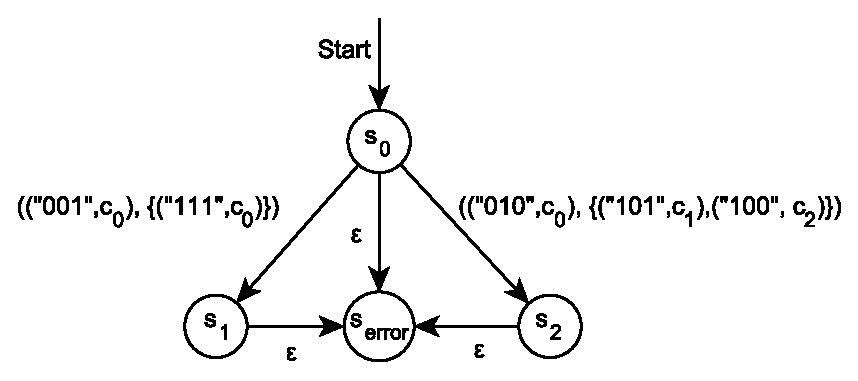
\includegraphics[scale=0.6]{figures/state-machines/simple-NFA.pdf}
		\caption{A simple example of our finite state machine model\label{fig:simple-nfa}}
	\end{figure}

	To show the transformation, we will model an arbitrary distributed protocol as consisting of \textit{finite state machines}, \textit{channels} and \textit{processes}.
	A finite state machine consists of a current state, $s_{current}$, a finite set of $n$ distinct states, $S=\{s_1, s_2, \dots, s_n\}$, and a finite set of $m$ distinct state-transitions, $T$.
	A finite state machine can only be in one state at any time, and transitions to another state by accepting a bit-string as input, and optionally outputs another bit-string. 
	A transition has the form $(s_{from}, i, o, s_{to})$, where $i$ is an input consisting of a tuple of a bit-string and the channel the bit-string was received on, and $o$ is the output consisting of a set of bit-string/channel pair, each representing that bit-string being sent on the appertaining channel.
	For example, the finite state machine in figure \ref{fig:simple-nfa} will transition from the starting state $s_0$ to $s_2$ on input $"010"$ from channel $c_0$, and will during the transition output $"101"$ to channel $c_1$ and $"100"$ to $c_2$.
	
	A channel can either be reliable or unreliable, and is bi-directional. 
	A reliable channel guarantees that messages sent on it will be delivered, will be delivered in the order the messages was sent, and will not be changed during transmission.
	An unreliable channel gives no such guarantees, and can thus experience loss, reordering and corruption of messages.

	The last component in our model is the process.
	A process is a set of running state machines.
	The state machines inside the process can be connected with reliable channels. 
	State machines can be connected to state machines in other processes only with unreliable channels.

	\begin{figure}[ht]
		\center
		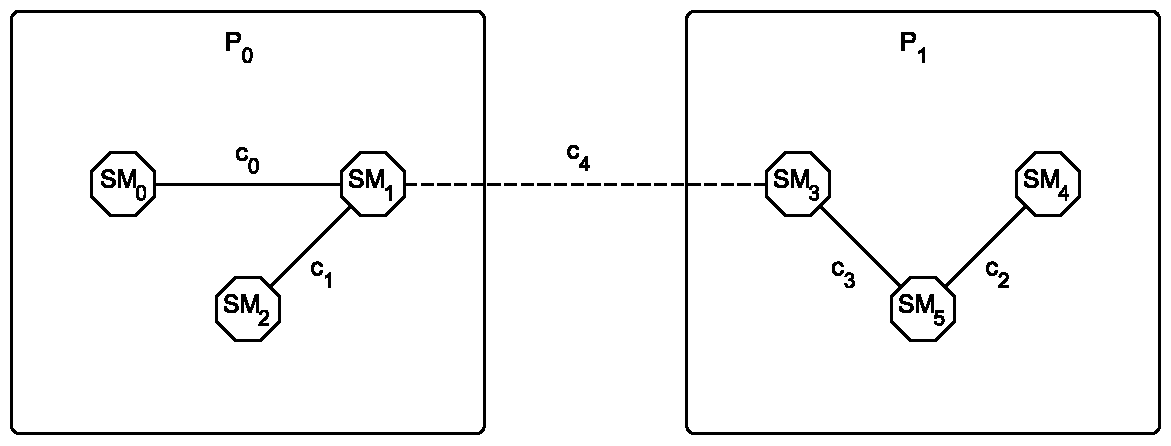
\includegraphics[scale=0.6]{figures/state-machines/Distributed-protocol-model.pdf}
		\caption{A simple example of distributed protocol model.\label{fig:simple-model}}
	\end{figure}

	Figure \ref{fig:simple-model} is a model of a simple distributed protocol, consisting of the processes $P_0$ and $P_1$, each of which has three state machines $SM_0 - SM_5$. 
	Each state machine is connected to other state machines on the same process with reliable channels $c_0-c_3$, and $SM_1$ on $P_0$ is connected to $SM_3$ on $P_1$ with the unreliable channel $c_4$.

	A distributed protocol can experience a plethora of different errors. 
	Apart from the channel faults already described, we will model crashes and byzantine faults, as these are the ones we are concerned about in this transformation.
	We model a crash fault in the state machine by adding an empty input transition ("$\epsilon$") from every state to an error-state, which cannot transition to another state (see $s_{error}$ in figure \ref{fig:simple-nfa}).
	As the state machine will not be able to transition to another state, and thus also cannot output anything from this state, this serves to model a component crashing in distributed protocol.
	We model a byzantine fault by exchanging a process with a new process.
	This potentially includes the removal of state machines, the addition of state machines or the exchange of old state machine with new state machines with new current states and new channels (we will refer to this last case as \textit{corrupted} state machines).
	This models a process beginning to exhibit arbitrary behaviour.

	To transform a crash-resistant distributed protocol into a byzantine-fault-tolerant protocol, we utilize the verification in Remote Attestation (see section \ref{subsec:attestation}) and the integrity guarantees provided by Intel SGX.
	To model the integrity guarantees, we introduce the notion of a cryptographic secret state machine $SM_{s}$, and an integrity protected area of the process.
	We assume that any byzantine fault can replicate $SM_{s}$, but cannot replicate the secrets contained in $SM_s$ if $SM_s$ is changed. 
	This models that faulty processes cannot access the cryptographic secrets of a correct process, which is a reasonable assumption by the integrity and confidentiality guarantees given by Intel SGX, given that the secrets are stored in an enclave (see section \ref{subsec:enclave}).
	State machines running in the integrity protected area of the process can be uniquely identified by $SM_{s}$, but cannot have channels to state machines running on other processes.
	This models the integrity protection in Intel SGX and the QE' abilities, as well as an enclave's inability to access peripheral hardware such as network cards.

	To model the Remote Attestation verification, we introduce a Remote Attestation process, $P_{RA}$ and an Attestation state machine, $P_A$, which will communicate with $P_{RA}$ to verify and provision $SM_s$ with a symmetric secret key.
	We will not go into detail with, or model the protocol used by, the Remote Attestation protocol, and just use it at an abstract for readability.
	For more information on the Remote Attestation protocol, see section \ref{subsec:attestation}, \textit{Intel SGX explained}~\cite{costan_intel_2016} and/or \textit{Intel SGX Developer guide}~\cite{intel_sgx_guide}.

	We will also assume that each process has a process unique identifier, $id_p$, that $SM_s$ knows $id_p$, and that each untransformed state machine includes both this $id_p$ and the $id_p$ of the intended receiver it's outgoing messages.
	In the case of broadcast messages, the $id_p$ of the receiving processes can be omitted. 
	In practise, this could be implemented as a process's external IP-address that is provisioned to $SM_s$ by in a verifiable or trusted manner (for instance by $P_{RA}$ during secret provisioning), or by a sufficiently large number that is randomly selected on process start up.
	Both of these solutions require a handshake protocol during channel establishment, in which $SM_s$ on each process must MAC their $id_p$ with the Remote Attestation provisioned secret for verification by the other process. 
	We will not describe this handshake protocol.

	The transformation from a crash-resistant protocol to a byzantine-fault-tolerant protocol consist of 4 steps on the process-level:
	\begin{enumerate}
		\item Add all the state machines to the integrity protected area of the process.
			\begin{itemize}
				\item This is equivalent to making the distributed components in the crash-resistant protocol into enclaves. 
				Please note that it is rarely necessary to make all components into enclaves, only the so-called \textit{security critical components}.
			\end{itemize}
		\item For each endpoint state machine in unreliable channels between processes, add a new state machine in the unprotected area of each of the processes (called a wrapper state machine), connect a new unreliable channel between these and add a reliable channel from the old endpoint state machines to the new.
			\begin{itemize}
			   	\item This is equivalent to adding unprotected wrapper components for the enclaves, which will have access to the network, an thus can act as a middle-man for communicating with other processes.
		    \end{itemize}
		\item Add reliable channels from all state machines in the integrity protected area of the process to the cryptographic secret state machine $SM_s$.
		\item Add an Attestation state machines, $SM_A$, to each process and a Remote Attestation process, $P_{RA}$ to the protocol.
	\end{enumerate}

	\begin{figure}[ht!]
		\center
		\includegraphics[scale=0.39]{figures/state-machines/distributed-protocol-model-transformation0.pdf}
	\end{figure}
	\begin{figure}[ht!]	
		\center
		\includegraphics[scale=0.39]{figures/state-machines/distributed-protocol-model-transformation1.pdf}
	\end{figure}
	\begin{figure}[ht!]	
		\center
		\includegraphics[scale=0.39]{figures/state-machines/distributed-protocol-model-transformation2.pdf}
	\end{figure}
	\begin{figure}[ht!]	
		\center
		\includegraphics[scale=0.39]{figures/state-machines/distributed-protocol-model-transformation3.pdf}
	\end{figure}
	\begin{figure}[ht!]	
		\center
		\includegraphics[scale=0.39]{figures/state-machines/distributed-protocol-model-transformation4.pdf}
		\caption{Transformation of figure \ref{fig:simple-model} from crash-resistant protocol to byzantine fault-tolerant protocol.\label{fig:tranformation-model}}
	\end{figure}
	\FloatBarrier

	The transformation of the state machines consists of the following:
	\begin{enumerate}
		\item Before a process runs the protocol, a pre-compute step must be added where each process' $SM_s$ is provisioned with the same cryptographic secret. 
		This is handled by the $SM_s$ and $SM_A$, which will contact $P_{RA}$ and be Attested and securely provisioned. 
		In our example, we have only added a single $P_{RA}$, which of course means that a \textit{k}-resilient protocol suddenly cannot handle a single $P_{RA}$ crash. 
		This can be solved by adding \textit{k+1} identical $P_{RA}$s, as this is a pre-compute step. 
		This means that the $P_{RA}$s plays no further role after this step in the protocol, and can crash without effecting the running processes.
		\item All messages that were to be sent in the original protocol, must be sent from a state machine in the integrity protected area though a state machine in the unprotected area of the process.
		This is due to the constraint that the state machines in the integrity protected area of the process can no longer have channels to other processes.  
		\item Before any message intended for another process is sent from the integrity protected area, it must be have a cryptographic message authentication code (MAC) appended on the message.
		The MAC is an output of the message and the Remote Attestation provisioned key.
		$SM_s$ is the only state machine with the Remote Attestation provisioned key, and thus only $SM_s$ can MAC a message correctly.
		$SM_s$ will refuse to sign any message if any state machine in the integrity protected area is not the original.
		This translates to a transformation of the state machine, such that each transition\\
		$(s_{from}, i, \{(m_o, c_o)\}, s_{to})$,\\
		where $c_o$ is a channel that was previously to another process, must be transformed to the transitions\\
		$(s_{from}, i, \{(m_o, c_{SM_s})\}, s_{wait})$ and\\ 
		$(s_{wait}, (m_o+MAC, c_{SM_s}), \{(m_o+MAC, c_o)\}, s_{to})$\\
		with the intermediate state $s_{wait}$, which acts as a state in which the state machine waits for $SM_s$ to MAC the output message.
		\item Whenever a message that supposedly originates from another process is received from the unprotected area  by a state machine in the integrity protected area, the MAC of that message must be verified by $SM_s$.
		In case this verification fails, the message must be dropped discarded.
		This translates to a transformation of the state machine, such that each transition\\
		$(s_{from}, (m_i, c_i), o, s_{to})$,\\
		where $c_i$ is a channel that was previously to another process, must be transformed to the transitions\\
		$(s_{from}, (m_i+MAC, c_i), \{(m_i+MAC, c_{SM_s})\}, s_{wait})$,\\
		$(s_{wait}, ("0", c_{SM_s}), \{\}, s_{from})$ and \\
		$(s_{wait}, ("1", c_{SM_s}), o, s_{to})$ \\
		with the intermediate state $s_{wait}$, which acts as a state in which the state machine waits for $SM_s$ to verify the MAC of the input, and the messages $"0"$ and $"1"$ represents the failure and success of this verification, respectively.
		\item In the event that $SM_s$ is asked to sign a message from a state machine that it identifies is not the original state machines in the integrity protected area, it must discard the message.
	\end{enumerate}

	Notice that this transformation is linear in the number of messages, under the assumption that the MAC, and MAC-verification sub-routines in $SM_s$ does not add any messages.
	Each input message in the transitions is transformed to exactly one new state, three new state transitions and one MAC-verification sub-routine on $SM_s$.
	Each output-set is transformed to exactly one new state, two new state transitions and $n$ MAC sub-routines on $SM_s$ where $n$ is the size of the output set.
	Under the assumption that $SM_s$ sends no additional messages during the MAC and MAC-verification sub-routines, and no failures, $m$ messages in the original state machine will become $7m$ messages after the transformation (see table \ref{tab:number-of-messages-transformed}).
	If we only count the messages sent between processes, there is no change in the number of messages sent.

	\begin{table}[ht!]
	\centering
	\makebox[\textwidth][c]{\begin{tabular}{l|l}
	\textbf{Number of messages} 	& \textbf{Origin} \\ \hline
	$m$                           	&  MAC-request outputs to $SM_s$                						\\ \hline
	$m$                           	&  MAC-response inputs from $SM_s$               						\\ \hline
	$m$                           	&  messages sent to the wrapper state machine on the sending process    \\ \hline
	$m$                           	&  messages sent between processes               						\\ \hline
	$m$                           	&  messages sent from the wrapper state machine on the receiving process               																					 \\ \hline
	$m$                           	&  input MAC verification requests to $SM_s$               				\\ \hline
	$m$                           	&  verification responses from $SM_s$                					\\ \hline\hline
	$7m$                          	&  total messages            
	\end{tabular}}
	\caption{Number of messages after the transformation}
	\label{tab:number-of-messages-transformed}
	\end{table}

	\FloatBarrier
	\begin{figure}[ht!]	
		\center
		\makebox[\textwidth][c]{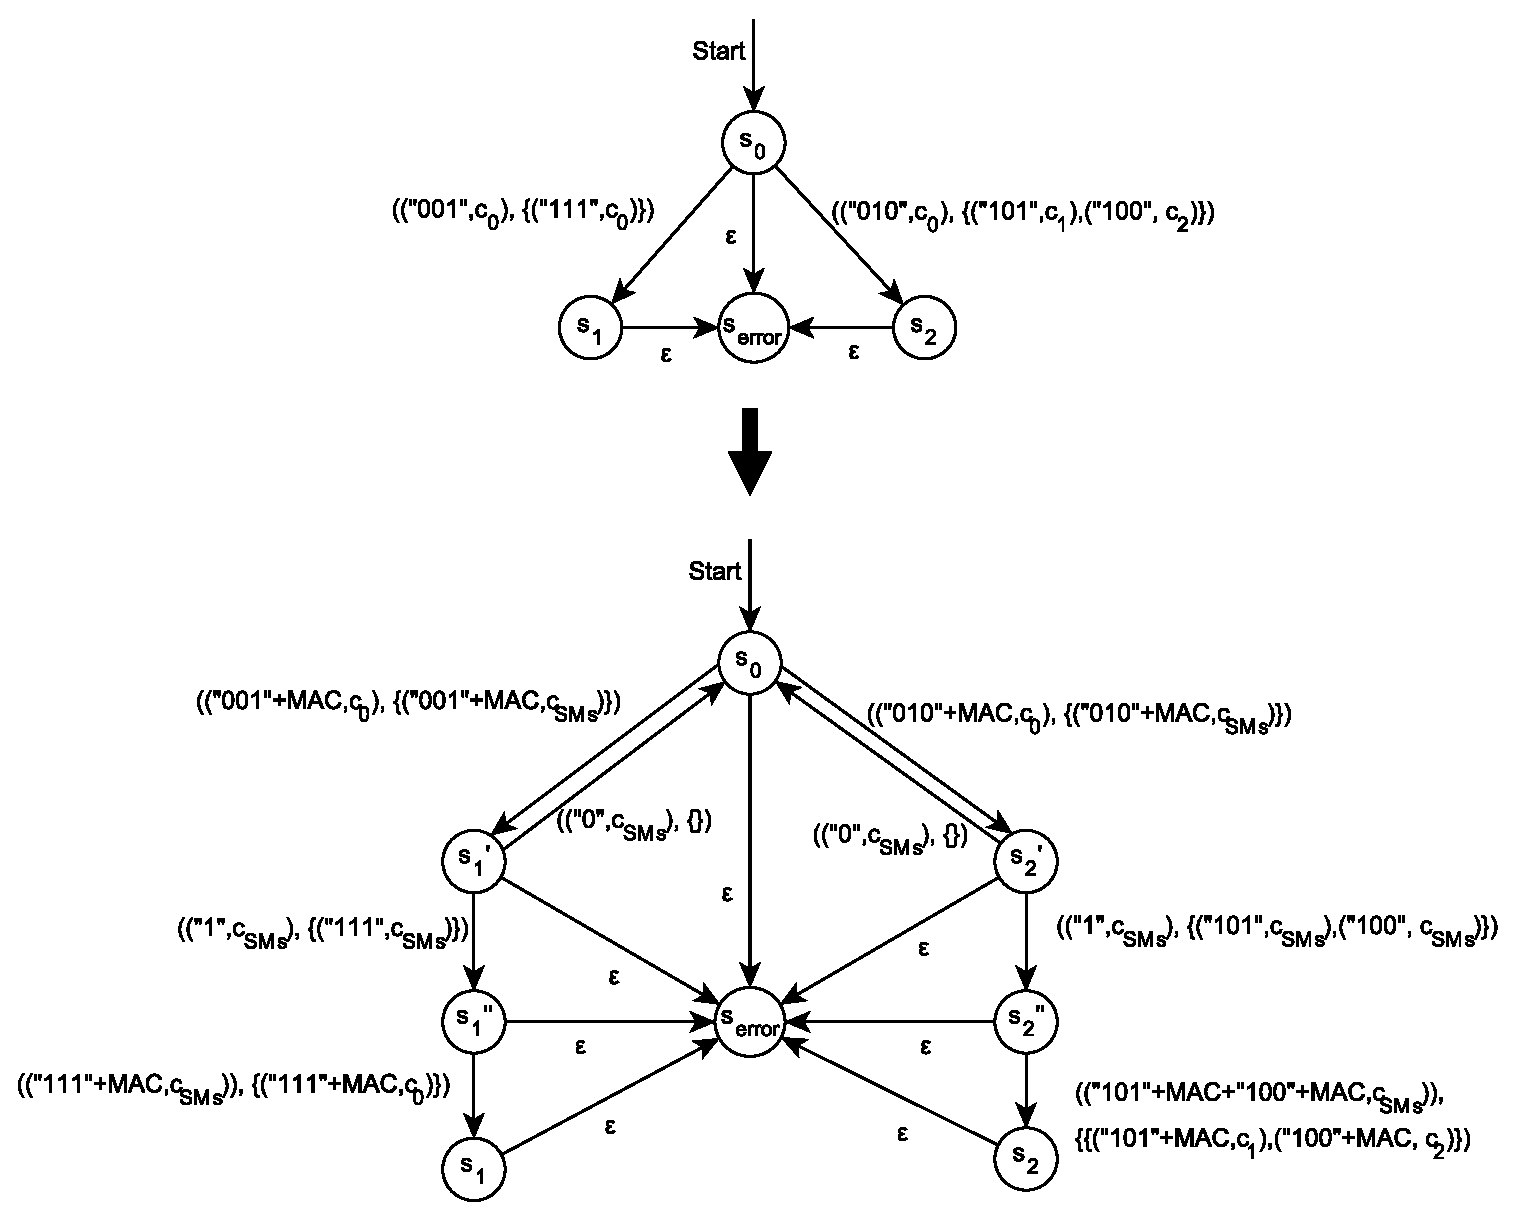
\includegraphics[scale=0.6]{figures/state-machines/NFA-transformation.pdf}}
		\caption{Transformation of figure \ref{fig:simple-nfa} from state machine in crash-resistant protocol to integrity protected state machine in byzantine fault-tolerant protocol, if all channels are to other processes.\label{fig:nfa-transformation}}
	\end{figure}
	\FloatBarrier

	These transformations gives us the following guarantees, if a process experiences a byzantine fault.
	Recall that we model a byzantine fault as a process being exchanged with a new process, potentially with removed, added and/or corrupted state machines.
	\begin{itemize}
		\item If a process has its transformed state machine removed, the process will exhibit exactly the same behaviour as a crash (the state machine can take no further inputs, and produce no further outputs), and so it is exactly equivalent to a crash of the state machine. 
		\item If the wrapper state machines are removed, the transformed state machine can no longer send or receive messages.
		This is again equivalent to a crash, as a token can no longer be sent to or from that state machine.
		\item If the $SM_A$ is removed, it can either happen before or after the Remote Attestation process has completed.
		If it happens before, the process's $SM_S$ will never be provisioned with the Remotely Attestation secret, and no messages will be verified.
		Therefore, the transformed state will never have its outgoing messages MAC'ed nor will it have any incoming messages verified.
		As such, it will either get stuck in a state where it never gets a response from $SM_s$ of a message MAC request, or it will get stuck in a state where a specific message cannot be verified.
		If it happens after the provisioning it will have no effect, as $SM_s$ is already provisioned, and no further communication with $SM_A$ is required.
		\item If a process gets an additional state machine in the integrity protected area, it will have no consequence, as $SM_s$ will refuse MAC'ing and verification of messages from this state machine, and it cannot communicate with other state machines, unless these are corrupted.
		\item If a process gets an additional state machine outside the integrity protected area, it cannot communicate with anything inside the integrity protected area, with corrupting these (see below). 
		It can communicate with other non-protected state machines, but this is equivalent to the other state machines being corrupted (see below).
		\item If a process has a corrupted transformed state machine (in the integrity protected area), $SM_s$ will refuse to sign any messages. 
		So any messages sent from this corrupted state machine, will not be verified on correct processes, meaning that the transformed state machines receiving this message will not transition any further than the verification state.
		\item If a process has a corrupted $SM_s$, the new $SM_s$ will, by assumption, not have access to the Attestation secret. 
		Thereby, it cannot MAC or verify messages.
		Nor can it be provisioned with the key again, as this the Remote Attestation procedure ensures that $SM_s$ is the correct state machine. 
		\item If a process has a corrupted wrapper state machine, any messages from the integrity protected area can either be dropped, changed/corrupted, redirected, or duplicated. 
		A dropped message is equivalent to a dropped message on an unreliable channel, which the protocol already handles.
		A corrupted message will not be verified by a correct receiving process's $SM_s$, and the message will be discarded.
		A redirected message will be not by verified by the receiving process, as it's $id_p$ will not match the intended recipient, and the message will be discarded.
		A duplicated message is equivalent to a duplicated message on the unreliable channel, which the protocol already handles.
	\end{itemize}
		
	This concludes the argument that Intel SGX and cryptography can change correct process behaviour under byzantine faults to behaviour equivalent that under crash faults, and thereby, using the above transformation, make a crash-resistant protocol into a byzantine-fault-tolerant protocol.
	As we will apply this transformation to our solution, we will therefore from here on in, only consider a fault model of crashing processes.

		\subsection{Example: Central Server Mutual Exclusion}
		We will now show a practical example of how the transformation in section \ref{sec:transforming-byzantine-faults} can be utilised.
		The protocol that we will transform is the central server protocol for mutual exclusion.
		The central server protocol for mutual exclusion (from here on in CSME) is a protocol which partly solves the \textit{distributed mutual exclusion} problem.
		In the distributed mutual exclusion problem, a collection of processes share one or more resources (referred to as the \textit{critical section}), and need to do read/writes on these resources. 
		To prevent race-conditions, a mutual exclusion algorithm ensures that only a single process has access to the critical section at any given time.
		More formally, in any solution to the distributed mutual exclusion problem, the following requirements must be upheld:
		\begin{description}
			\item[ME1: Safety] At most one process may execute in the critical section (CS) at a time.
			\item[ME2: Liveness] Requests to enter and exit the critical section eventually succeed.
		\end{description}
		Optionally, some distributed mutual exclusion protocols also solves the additional fairness requirement of
		\begin{description}
			\item[ME3: Happened-before ordering]  If one request to enter the CS happened-before another, then entry to the CS is granted in that order. 
		\end{description}
		CSME does not fulfil the requirements of ME3 in asynchronous systems, and thus only partly solves the distributed mutual exclusion problem.

		CSME solves ME1 and ME2 under the conditions of no process failures.
		In broad strokes, the protocol works by deploying a central server process, which will process a request for access to the critical section in the received order, send an access token to the appropriate client process, waits for an acknowledgement from the process that access to the critical section is no longer needed, and then processes the next request.
		It is trivial that the protocol does not provide liveness under process crashes:
		If the server crashes, no process can gain access tokens, and thus no requests for access will succeed.
		The same scenario is true if a process crashes while having access to the critical section, as the server will never release the token of the crashed process.
		However, safety is still guaranteed, as a process cannot access the critical section without a token.
		Under byzantine faults, neither safety nor liveness can be guaranteed. 
		For instance, the server could serve the tokens to all requests without waiting for acknowledgements from the clients.

		We will now show how the transformation from section \ref{sec:transforming-byzantine-faults}, can transform CSME to give the same guarantees in a byzantine system as the untransformed protocol gives in a crash-fault system.
		Notice that there is no formal definition of how the critical section access and token is implemented in CSME -- it can be implemented with cryptography, as partial states, with append-only memory, as another process, etc.
		We will keep this abstraction in the following transformation, but the implementation of this is also required to undergo the same transformation.
		We will omit the handling of unreliable channels on the state machines for readability, but assume that it is handled.

		First we need to model the protocol as finite state machines, channels and processes.
		We model two different state machines: a client state machine, and a server state machine.

		\FloatBarrier
		\begin{figure}[ht!]	
			\center
			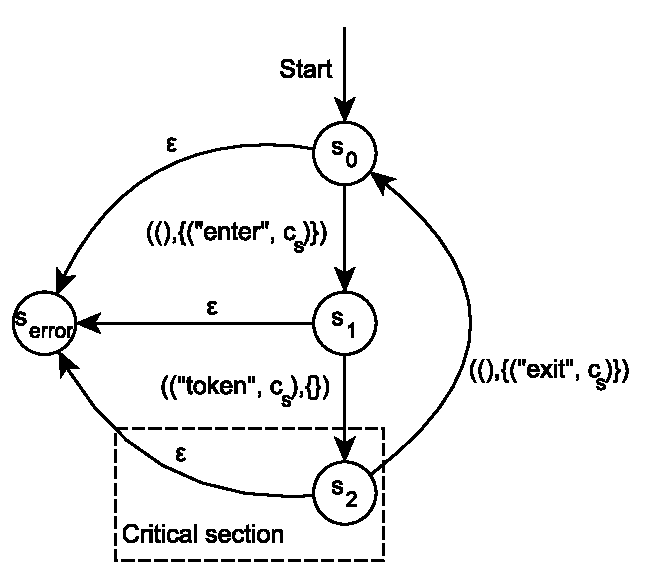
\includegraphics[scale=0.6]{figures/state-machines/CSME-client-NFA.pdf}
			\caption{Client state machine from the central server protocol for mutual exclusion. Note that the channel $c_s$ represents the unreliable channel to the server, and is different across client instances.\label{fig:CSME-client-NFA}}
		\end{figure}
		\FloatBarrier

		The client state machine is quite simple, and is modelled in figure \ref{fig:CSME-client-NFA}.
		It can either not not have requested access to the critical section ($s_0$), wait for the token from the server ($s_1$), or have the token and be in the critical section ($s_2$). 
		Naturally it can also crash ($s_{error}$).

		\FloatBarrier
		\begin{figure}[ht!]	
			\center
			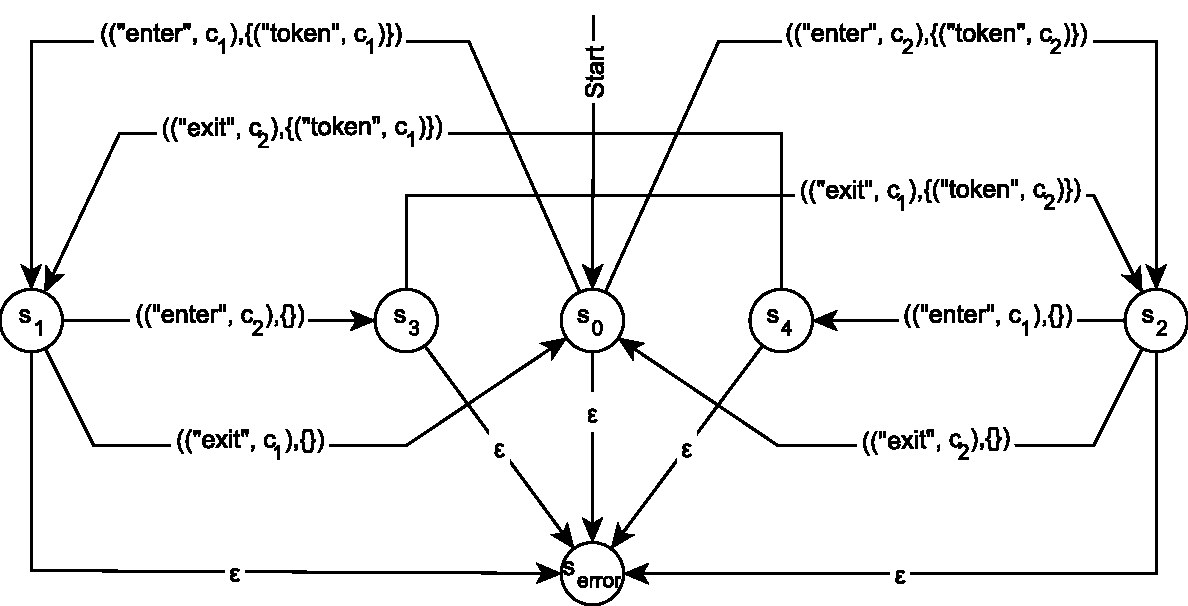
\includegraphics[scale=0.6]{figures/state-machines/CSME-server-NFA.pdf}
			\caption{Server state machine from the central server protocol for mutual exclusion. Note that this server state machine can only handle two client processes.\label{fig:CSME-server-NFA}}
		\end{figure}
		\FloatBarrier

		The server state machine is a bit more complex as it must be modelled to account for the number of client processes.
		Figure \ref{fig:CSME-server-NFA} is a model of the server state machine in a protocol with two client processes.
		It encompasses 6 states: $s_0$ where no client has access to the critical section, and no requests has been , $s_1$ where client $1$ has requested the token and the token has been sent, $s_2$ where client $2$ has requested the token and the token has been sent, $s_3$ where client $1$ has the token and client $2$ has requested the token, $s_4$ where client $2$ has the token and client $1$ has requested the token and $s_{error}$ where the state machine has crashed.

		\FloatBarrier
		\begin{figure}[ht!]	
			\center
			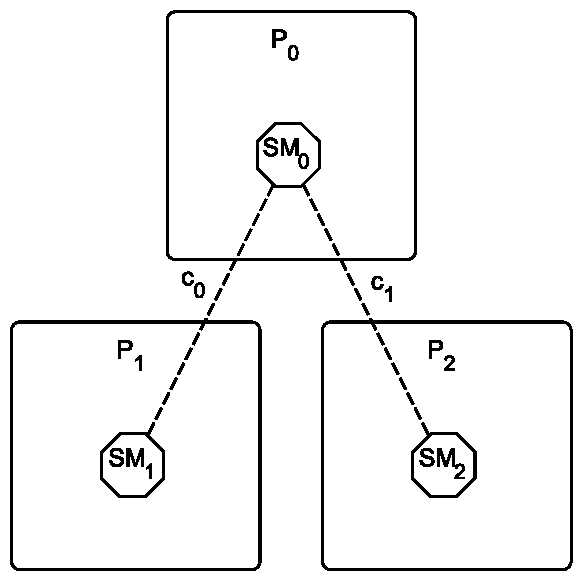
\includegraphics[scale=0.6]{figures/state-machines/CSME-protocol.pdf}
			\caption{Processes and channels in the central server protocol for mutual exclusion, with one server and two clients.\label{fig:CSME-protocol}}
		\end{figure}
		\FloatBarrier

		Figure \ref{fig:CSME-protocol} show the processes and channels in CSME with two client processes.
		$P_1$ and $P_2$ are the clients, each running an instance of the state machine from figure \ref{fig:CSME-client-NFA}, with an unreliable channel to the server process $P_0$, which runs an instance of the state machine from figure \ref{fig:CSME-server-NFA}.

		We start the transformation by transforming the state machines to have their messages MAC'ed by $SM_s$, and to have $SM_s$ verify the messages they receive.
		This is done by rules for state machine transformation in section \ref{sec:transforming-byzantine-faults}. 

		\FloatBarrier
		\begin{figure}[ht!]	
			\center
			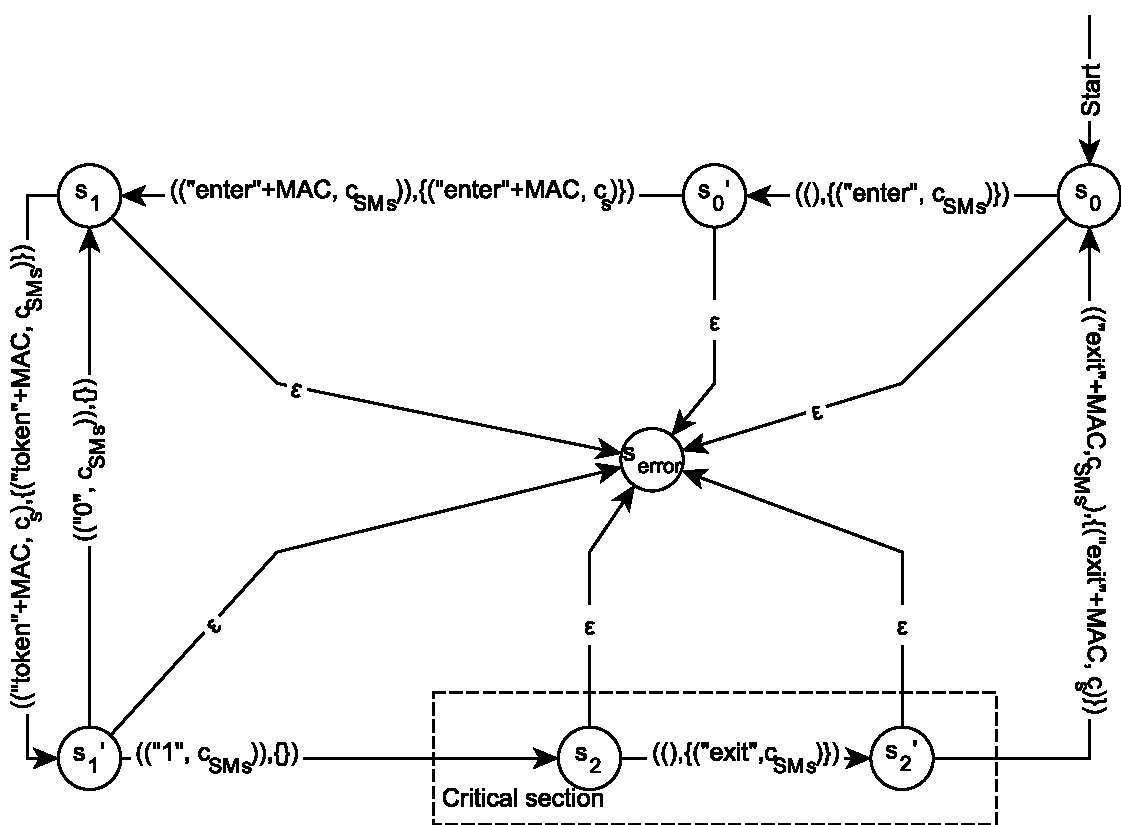
\includegraphics[scale=0.6]{figures/state-machines/CSME-client-NFA-transformed.pdf}
			\caption{Client state machine in CSME, after it has been transformed to handle byzantine faults.\label{fig:CSME-client-NFA-transformed}}
		\end{figure}
		\FloatBarrier
s
		Figure \ref{fig:CSME-client-NFA-transformed} shows the client state machine after the transformation.
		Whenever the client wants to enter the critical section, the state machine sends the request to $SM_s$ for MAC'ing.
		When the MAC'ed message is received from $SM_s$, this message is sent to the server process. 
		The state machine is now in $s_1$, which is equivalent to $s_1$ in the untransformed state machine (figure \ref{fig:CSME-client-NFA}).
		$c_s$ is now a channel from the wrapper state machine.
		When a token is received from $c_s$, the message's MAC is sent to $SM_s$ for verification.
		If the MAC is correct, the state machine will transition to $s_2$, which is in the critical section, and is equivalent to $s_2$ in the untransformed state machine.
		Before exiting the critical section, the exit message is sent to $SM_s$ for MAC'ing, and when the appropriate MAC is received from $SM_s$, the exit message is sent to the wrapper state machine for redirection to the server process.

		\FloatBarrier
		\begin{figure}[ht!]	
			\center
			\makebox[\textwidth][c]{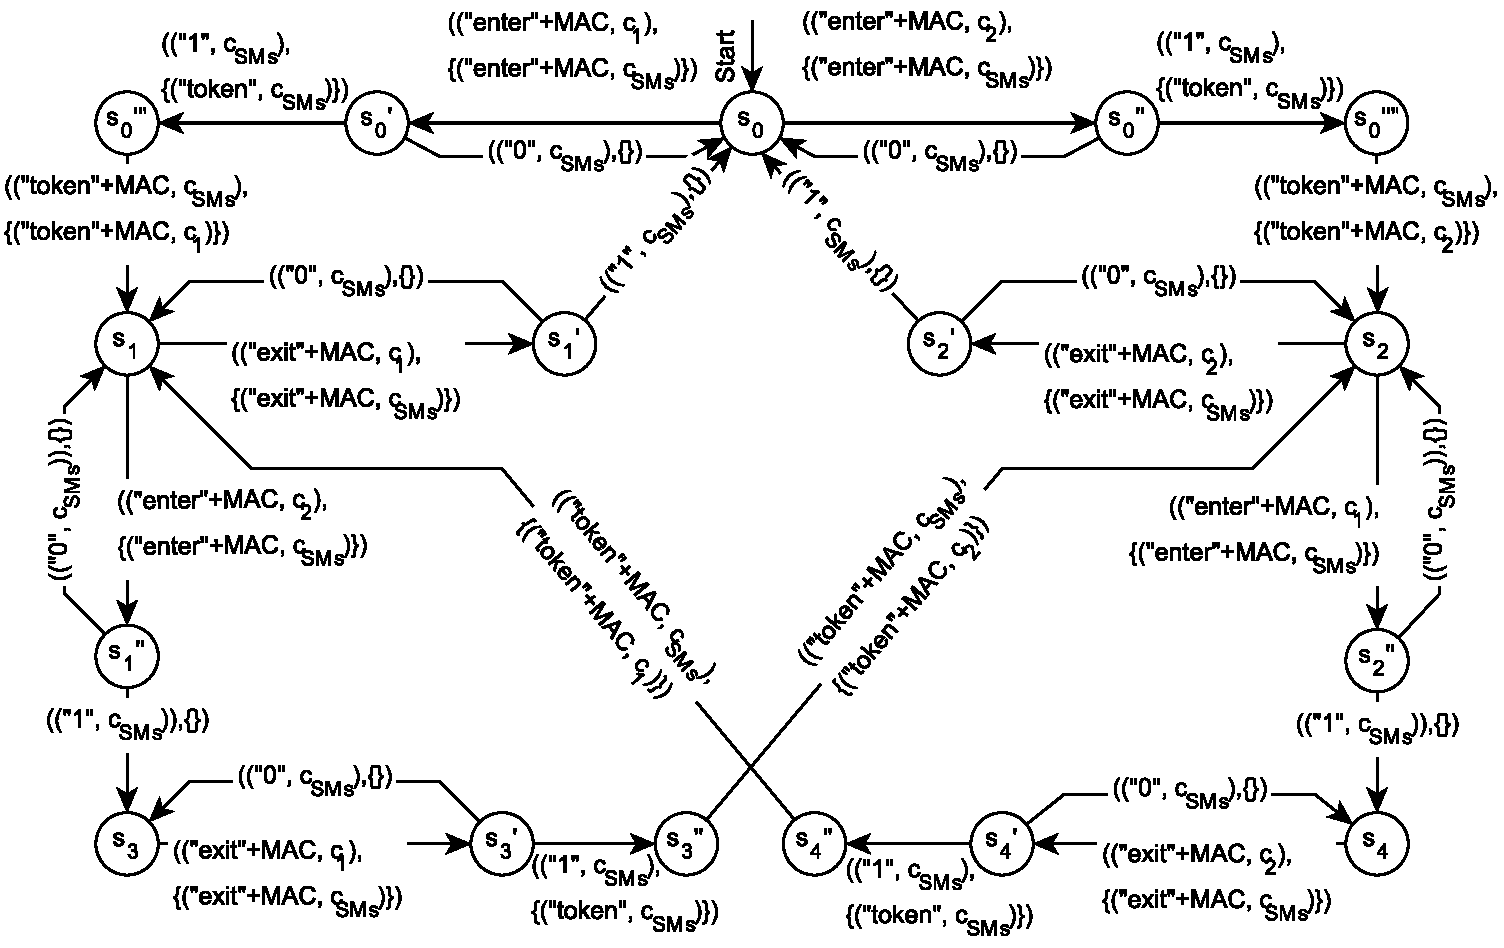
\includegraphics[scale=0.6]{figures/state-machines/CSME-server-NFA-transformed.pdf}}
			\caption{Server state machine in the central server protocol for mutual exclusion, after it has been transformed to handle byzantine errors. Note that $s_{error}$ has been omitted for (some) readability.\label{fig:CSME-server-NFA-transformed}}
		\end{figure}
		\FloatBarrier

		Figure \ref{fig:CSME-server-NFA-transformed} shows the transformed server state machine.
		We have omitted $s_{error}$ for readability.
		$s_0$, $s_1$, $s_2$, $s_3$ and $s_4$ are equivalent to the states by the same names in the untransformed state machine (figure \ref{fig:CSME-server-NFA}).
		In $s_0$ the token has been released, and no client has requested the token.
		In $s_1$, client $1$ has requested the token, $SM_s$ has verified the MAC of the request and MAC'ed the token which has then been sent to the servers wrapper state machine for redirection to the client $1$ process.
		If the token is released by client $1$, and this message's MAC is verified, the state machine will transition to $s_0$. 
		$s_2$ is equivalent to $s_1$, except with client $2$ instead of client $1$. 
		In $s_3$, client $1$ has the token, and client $2$ has requested the token.
		So when the server state machine receives a verifiably "exit" message from client $1$, a token is MAC'ed and sent to client $2$, so the state machine can transition to $s_2$.
		$s_4$ is equivalent to $s_3$, except with the clients reversed (client $2$ has the token, client $1$ has requested it, when client $2$ releases the token).  

		\FloatBarrier
		\begin{figure}[ht!]	
			\center
			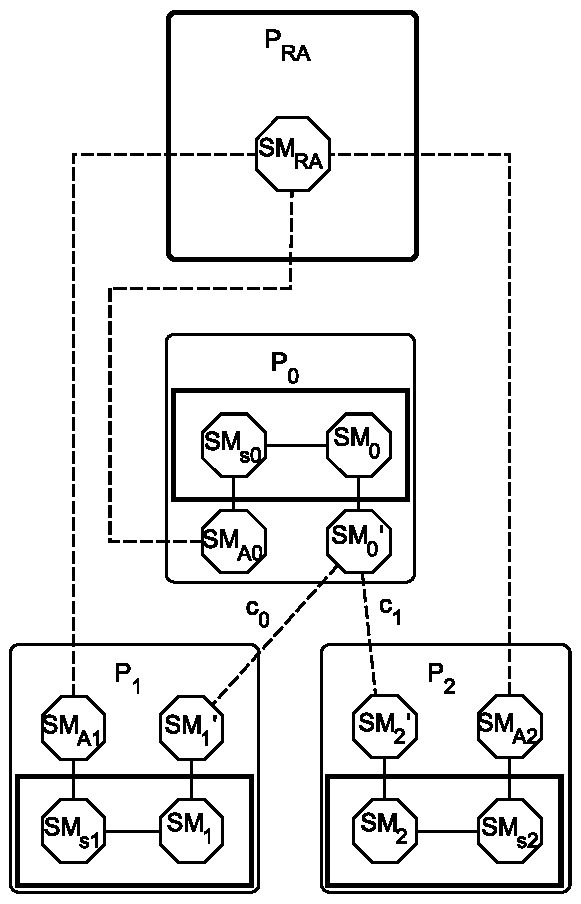
\includegraphics[scale=0.6]{figures/state-machines/CSME-protocol-transformed.pdf}
			\caption{Processes and channels in the central server protocol for mutual exclusion, after they have been transformed to handle byzantine errors.\label{fig:CSME-protocol-transformed}}
		\end{figure}
		\FloatBarrier

		Figure \ref{fig:CSME-protocol-transformed} show the process's transformation. 
		Each of the client processes ($P_1$ and $P_2$), is now running the transformed client state machines in the integrity protected area. The transformed client state machines have a reliable channel to a $SM_s$, and another to a wrapper state machine outside the integrity protected area, which is responsible for passing on the messages to the server process.
		Each of the processes have has an $SM_A$ responsible for passing Remote Attestation messages from the $SM_s$ to the new Remote Attestation process.
		The server process is running a transformed server state machine, connected to two wrapper state machines and an $SM_s$.
		The server $SM_s$ is also connected to a $SM_A$ for attestation.

		Having transformed the CSME protocol, the correct processes will exhibit the same behaviour when other processes suffer byzantine faults, as the correct processes do in the untransformed protocol when other processes suffer crash faults.

		\FloatBarrier
		\begin{figure}[ht!]	
			\center
			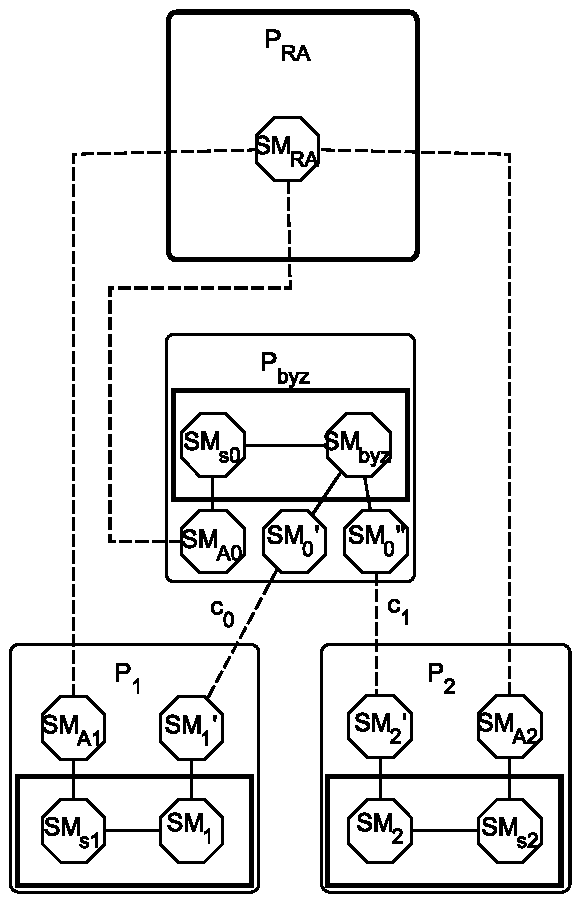
\includegraphics[scale=0.6]{figures/state-machines/CSME-protocol-transformed-byzantine.pdf}
			\caption{Processes and channels in the transformed central server protocol for mutual exclusion, with a byzantine fault on the server process.\label{fig:CSME-protocol-transformed-byzantine}}
		\end{figure}
		\FloatBarrier

		Let's see how a byzantine fault is reduced to a crash failure in the example where the server state machines tries to serve tokens on any request, without getting acknowledgement that the token has been released by the possessing client.
		There are several ways this could be modelled, one of which is presented here:
		We model this byzantine fault as $P_0$ being exchanged with $P_{byz}$.
		$P_{byz}$ (see figure \ref{fig:CSME-protocol-transformed-byzantine}) is exactly equal to $P_0$, except that $SM_0$ has been exchanged with $SM_{byz}$ (see figure \ref{fig:CSME-server-NFA-transformed-byzantine}), which serves a token to any request by the clients.

		\FloatBarrier
		\begin{figure}[ht!]	
			\center
			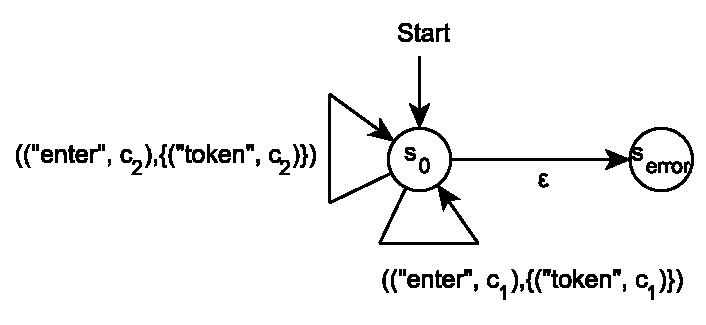
\includegraphics[scale=0.6]{figures/state-machines/CSME-server-NFA-transformed-byzantine.pdf}
			\caption{The byzantine fault state machine $SM_{byz}$ on the server process.\label{fig:CSME-server-NFA-transformed-byzantine}}
		\end{figure}
		\FloatBarrier

		If this byzantine fault happens, none of the tokens are MAC'ed.
		Thereby, any correct client process (figure \ref{fig:CSME-client-NFA-transformed}) will get stuck in a loop between $s_1$ and $s_1'$, when $SM_s$ rejects the (missing) MAC of the token. 
		This is equivalent behaviour to the server process crashing, as a (correct) token will never be provided, and the client is unable to enter the critical section.

	\section{Analysis}
	\label{sec:analysis}

	Consider a solution where a DCR graph is distributed among peers, such that each peer is responsible for one or more events.
	Responsible meaning that that peer maintains the state of that event along with the other peers responsible for the same event.
	Effectively, responsibility entails involvement in executions of the event and executions of event which could affect that event, as the state of the event must be agreed upon by all responsible peers.

	Any client can contact a peer, requesting an execution of an event, provided that that client has the correct credentials, with regards to access control.
	The first issue thereby presents itself, in that simultaneous client requests can lead to execution of dynamically dependent events.
	Since the executed events are dependent, the order in which the executions are attempted is not inconsequential, as they can be mutually exclusive, or dependent on one another, such that one can be executed followed by the other, but not vice versa.
	To solve this, the involved parties must agree on which order these executions are applied, to avoid inconsistencies in the state of the events.

	Synchronizing state changes is a well-known problem and one solution is the election of a leader which orders the messages, such as in most BFT algorithms~\cite{castro_practical_1999,veronese_efficient_2013,kapitza_cheapbft_2012,liu_scalable_2016}.
	%A single-leader system does however neccesitate that each peer in the system manages the entire subject state | in the case of this project the entirety of the DCR graph.
	\begin{table}[!ht]
	\centering
	
	\makebox[\textwidth][c]{\begin{tabular}{|p{0.2cm}|p{1.5cm}|p{1.5cm}|p{1.7cm}|p{2cm}|p{2cm}|p{1.5cm}|}
	\hline
	\#   & Fault tolerance (Availability) & Fault tolerance (Safety) & Fault tolerance (Data loss) & Nb. of messages for state change (Best case)       & Concurrency           & Request Bottleneck    \\ \hline
	\textit{1} & $0$                            & n/a ($0$)                & $0$                         & $2$                                                & None                  & $S$                   \\ \hline
	\textit{2} & $f$                            & $n$                      & $n$                         & $2(f+1)$                                           & Total                 & $L$                   \\ \hline
	\textit{3} & $\frac{(m-1)}{2}$ (partly)     & $n$                      & $m-1$                       & $2\frac{(m-1)}{2}$                                 & Total                 & $L$                   \\ \hline
	\textit{4} & $\frac{(m-1)}{2}$ (partly)     & $n$                      & $m-1$                       & $2\frac{(m-1)}{2}$                                 & Up to DCR concurrency & $L \cdot \frac{n}{m}$ \\ \hline
	\textit{5} & $0$ (partly)                   & $n$                      & $0$                         & $2 \cdot D_{dyn}(G,e)$ 							  & Up to DCR concurrency & $L$                   \\ \hline
	\end{tabular}}
	\caption{Comparison of different approaches.
	1: Central Server.
	2: State Machine Replication.
	3: Event state distributed and replicated with full consensus.
	4: Event state distributed and replicated with dependency consensus.
	5: Event state distinctly distributed (2PC).}
	\label{tab:approcach-comparison}
	\end{table}

	%Having a single leader is, however, not possible while fulfilling the requirements specified in this thesis, as it does not allow a distribution of state.

	To avoid the high number of messages associated with a fully replicated system and the message bottleneck associated with a single-leader system, we propose a multi-leader, partial state system with the following components:


	This algorithm solves the problem with performing locking before committing, leading to the first key problem of the algorithm:
	\begin{description}
		\item[Locking] When an event is executed, synchronization with the affected events by locking must be enforced, in order to avoid incompatible transactions.
		As locking is expensive both in regards to concurrency and the number of messages required, a minimal number of locks is desired.
		This issue is therefore concerned with how far changes from an event execution can propagate, necessitating locking, and whether or not there are identifiable cases where locks can be spared.
	\end{description}

	The second problem is closely related as consensus must be achieved on which peer holds which lock:
	\begin{description}
		\item[Consensus] In extension to preventing simultaneous incompatible executions, locking has pushed the issue of concurrency into the locking portion, which now needs to be handled in the sense that peers must agree on who holds the locks.
		Existing solutions to this problem, such as BFT algorithms and State Machine Replication Algorithms could be applied here, if each peer is responsible for the entirety of the graph.
		However, as those algorithms they are typically quite costly, as discussed earlier, they do not live up to the requirements specified in this thesis.
	\end{description}
	
	With solutions to the problems of locking and consensus, peers are able to progress the graph, but since they will not necessarily be aware of the state of the graph, they would have to aggressively push for an execution for it to possibly happen.
	This brings us to the problem of obtaining the global state of the graph:
	\begin{description}		
		\item[Global state collection] Each peer must be able to, at any time, collect a global state of the graph, with the guarantee that that global state will never be invalidated by a global state collected in the future.
	\end{description}

	As this is a decentralized peer-to-peer network solution, two key points also have to be considered:
	\begin{description}
		\item[Network topology] As the weakest point of the graph will be the event with the fewest peers responsible for it, some consideration must be given to what, if any, events are to be prioritized.
		Otherwise some distribution must be specified.
		\item[Peer distribution] As events only lock other events in the vicinity, something could be gained, performance-wise, by distributing the events such that they are responsible for events that would typically be locked during the same execution.
	\end{description}

	\subsection{Locking} % Missing a conclusion: When do we lock what? We have only described cases but not what our locking algorithm is.
	\label{subsec:locking}
	As discussed in section \ref{sec:analysis}, the execution of non-independent events must be synchronised.
	This is achieved through locking of individual events.

	For this section, we apply terms used in directed graphs and define variations of neighbourhoods with regards to DCR graphs as:
	\begin{description}
		\item{Neighbourhood}
		\item[Out-neighbourhood] denoted $N_{out}(v)$ and defined as the set of relations targeting the event $v$.
		\item[In-neighbourhood] denoted $N_{in}(v)$ and defined as the set of relations originating from the event $v$.
	\end{description}
	For all definitions of neighbourhoods, we denote it as closed or open, if it includes the event $v$ or not, respectfully. \\
		
	In a graph, $G(E,V)$, we define the set of locked events, $L$, on the execution of an event, $v$, as $L(v)$.
	As DCR only allows the execution of an activity to affect events in the neighbourhood, and that neighbourhoods neighbourhood, of the executing event, locking need only be performed within this set.
	Locking can be performed on the entirety of $L(v)\ =\ N(N(v))\ \cup\ N(v)\ \cup\ v$ on the execution of $v$, guaranteeing synchronization in the case of competing event executions.
	However, since locking two neighbourhoods actually gives a range of four, locking some subset could be just as correct and more efficient.

	\begin{figure}[ht!]	
		\center
		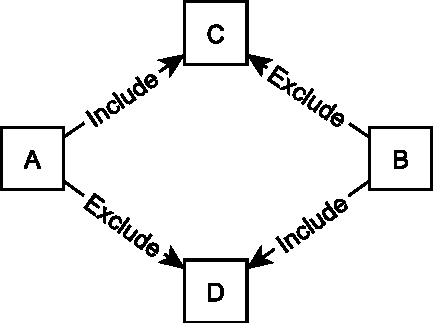
\includegraphics[scale=0.5]{figures/dcr-graphs/race-condition.pdf}
		\caption{Graph illustrating the need for locking within $N_{out}(v)$.}
		\label{fig:race-condition}
	\end{figure}

	In the graph shown in figure \ref{fig:race-condition} it is shown that at least part of the locking set has to be $N_{out}(v)$ so as to avoid a race condition in this case.

	\begin{figure}[ht!]	
		\center
		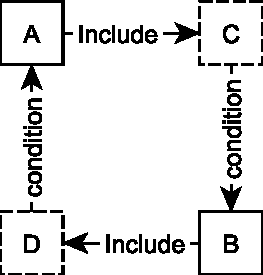
\includegraphics[scale=0.5]{figures/dcr-graphs/second-degree-effect.pdf}
		\caption{Graph illustrating the need for locking in either $N_{out}(N_{out}(v))$ or $N_{in}(v) \cup N_{out}(v)$.}
		\label{fig:second-degree-effect}
	\end{figure}

	In the graph shown in figure \ref{fig:second-degree-effect} it is shown that the locking set has to include either $N_{out}(N_{out}(v))$ or $N_{in}(v) \cup N_{out}(v)$, in order to prevent the graph from ending in a state where both \texttt{A} and \texttt{B} has been executed, which should be impossible due to the execution of either including a condition on the other.

	\begin{figure}[ht!]	
		\center
		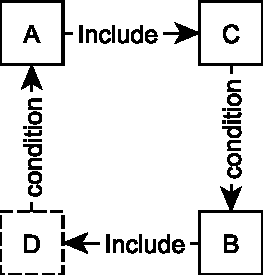
\includegraphics[scale=0.5]{figures/dcr-graphs/second-degree-no-effect.pdf}
		\caption{Graph illustrating the advantage of locking in $N_{out}(N_{out}(v))$ rather than $N_{in}(v) \cup N_{out}(v)$.}
		\label{fig:second-degree-no-effect}
	\end{figure}

 	In the graph shown in figure \ref{fig:second-degree-no-effect} an execution of \texttt{A} no longer has an effect on the enabledness of \texttt{B}, as \texttt{C} has the same state before and after the execution of \texttt{A}.
 	If the locking scheme of $L(v) = N_{in}(v) \cup N_{out}(v) \cup v$ is applied, this has no effect, but if the locking scheme of $L(v) = N_{out}(N_{out}(v)) \cup N_{out}(v) \cup v$ is used, the lock on \texttt{B} can be foregone.
	This optimization is, however, only possible when the state of \texttt{C} is known and since locking is only performed forwards, there is no implicit way to propagate executions backwards.
	This means that \texttt{A} does not know the state of \texttt{C} on execution and would have to do one of two options when executing:
	\begin{itemize}
		\item \texttt{A} sends a locking message to \texttt{C}, telling it to lock \texttt{B} if necessary.
		\item \texttt{A} sends a locking message to \texttt{C} and one to \texttt{B}, but gives \texttt{B} the option to forgo locking if the state of \texttt{C} would be unchanged by the execution of \texttt{A}.
	\end{itemize}
	Both options result in the minimum amount of locks, but the first option has fewer messages, as it only results in two messages.
	However, the first option has the disadvantage of potentially taking twice as long, assuming that transporting a message between \texttt{A} and \texttt{C} takes the same amount of time as between \texttt{A} and \texttt{B}.
	These various advantages of different methods means that finding one optimal solution is not possible, as it is dependent on the specific workflow and the topology of the network at a given time. 

	\subsection{Consensus} % Probably a bad name? Should contain description of messages, lamport diagrams, requirements for when to commit/abort, etc.

	% \subsection{Network topology}
	% Due to the algorithm not requiring the executioner of an event to have the global state of the workflow at the time of execution, any state changes are only propagated to the relevant parties.
	% This means that any single crash could potentially make collecting the global state, or history of executions, impossible, as the localized state of the crashed peer would be lost.
	% To make the system more tolerant to crashes, the state of each event is tracked by a number of peers.
	% This means that all locks need to be made on a subsystem rather than a single peer.
	% As this lock needs to prevent others from locking simultaneously, $\dfrac{m}{2} +1$ locks are required for each peer, where $m$ is the number of peers tracking the state of that event.

	% \subsubsection{Peer distribution}
	% Given that the relations of a workflow are fixed at creation, the peers can be distributed efficiently by assigning events frequently locked simultaneously to the same peers.
	% This can be accomplished by the following steps:
	% \begin{itemize}
	% 	\item Each event is assigned a set of peers, called the primaries of that event, containing at least one peer.
	% 	\item The primaries of each event are added to each event on which the execution of the event tracked by the primaries could incur a lock. The peers added this way are called secondaries for that event.
	% \end{itemize}

	% The peer-to-peer network is then configured in such a way that each peer is a neighbour to any peer which tracks the same events.
	% This means that the execution of an event can be performed by a primary, by that primary attempting to lock all of its neighbours and checking whether or not the acquired locks are sufficient in order to perform the execution, meaning that the set of locked peers forms a quorum for each event requiring a lock.

	% Crash recovery

	% \subsection{Message composition}
	% In order to reduce the amount of messages needed in the system, the locking of an event can incorporate. 

	\subsection{Global state collection}
	Because of the way that changes are propagated through the network, at no point can the state of the entire workflow be ascertained.
	Both as documentation of the process at deprecation of the workflow and during the life cycle of the workflow, the global state is relevant.
	This means that there needs to be some method of collecting the state at any given time.
	Due to the locking portion of the algorithm and the assumed absence of byzantine failures, except for crashes, collecting the state is as simple as requesting it from every peer in the network.
	As long as enough peers respond so that a quorum of states has been obtained for each event, all successful executions performed before the state collection algorithm was started, have been recorded.
	There is however an issue in that each event will then have their individual perceived sequence of executions, which might be dissimilar due to arbitrary message delays.

	Consider a simple graph of two events with a condition between them: $\ev{A} \crel \ev{B}$
	If a global state collection is started, originating at \texttt{A} after which \texttt{A} and then \texttt{B} is executed, the collection of the global state would return an empty sequence from \texttt{A} and a sequence of $\{\texttt{A}, \texttt{B}\}$ from \texttt{B}.
	This means that the global state collected by this would be the sum of returned sequences: $\{\texttt{A}, \texttt{B}\}$

	There are however situations where this is insufficient, as it is not always clear how to aggregate the returned sequences.
	Consider the graph: $\ev{A} \erel \ev{B}, \ev{B} \crel \ev{C}, \ev{D} \irel \ev{B}$
	On the first execution of \texttt{A}, \texttt{C} is notified, but since subsequent executions do not need to lock \texttt{C} due to \texttt{B} being unaffected by them, \texttt{C} will only be notified once.
	If \texttt{D} is also executed after \texttt{A} has been executed, then it is unclear how a combined history of executions would look like, as there are multiple valid points in the sequence for the execution of \texttt{C}.

	The ordering of these messages can therefore not be trivially achieved.
	To solve this, each event attaches the value of a monotonic counter\footnote{starting at 0} to each execution of that specific event.
	This makes multiple executions of an event indistinguishable from one another and means that the ordering can be deterministically achieved and that only executions performed during a global state collection can possibly be in the resulting collected state.

	Even though the executions can be ordered at any given time, there is the possibility of this ordering changing depending on which peer attempts to collect the global state.
	This is possible due to the locking system regarding some events to be concurrent (as described in REF), as the execution of those events have no competing locks.

	\section{Security analysis}
	The following is a security analysis of the algorithm described in section~\ref{sec:algorithm}.

		\subsection{Adversary model}
		We allow for a very strong adversary that can coordinate faulty nodes, delay communication and delay correct nodes, but not indefinitely. 
		We assume that the adversary is computationally bound, so that they are probabilistically unable to subvert the cryptographic techniques described above.
		
		\subsection{Analysis}
		
	\section{DCR-TEE Implementation}

	\section{Distributed Smart Contract Engine}

	\section{Discussion}

		\subsection{SGX security}
	    All aforementioned hardware guarantees are given by Intel, but since very little of the proprietary technology is documented, all security properties of SGX rely on the correctness of Intel's hardware implementation.
	    Historically Intel has had vulnerabilities in similar hardware components, like the CVE-2017-5689 security incident exposed in~\cite{silent_bob}, allowed unprivileged access to the Intel Active Management Technology.

	    SGX claims to provide confidentiality and integrity for running enclaves.
	    This is ensured by preventing untrusted software access to the PRM and enclaves access to other regions of the PRM besides their exclusive region.
	    However, while it is not possible to breach the integrity of PRM,~\cite{costan_intel_2016} shows several issues regarding confidentiality.
	    Because enclaves use the system page table even for data residing on PRM, it is possible for untrusted software to learn the page access order by manipulating the OS controlled page table.
	    Another possible attack vector is to perform cache timing by cleverly choosing the physical memory position of enclave memory pages on set associative caches.
	    By mapping snooping software to the same cache set as the enclave, the snooping software can evict the enclave's memory from the cache and use timing to figure out if it is accessed again.
	    Lastly, processors with hyper-threading support are vulnerable to instruction snooping, as a snooping process sharing physical core with an enclave can use performance counters to determine which instructions the out-of-order scheduler is able to run in parallel with the enclave.
	    The presence of these attacks means that enclaves using data-dependent memory access will likely not ensure confidentiality.
	    However, to our knowledge, no publicly known vulnerabilities exist on the integrity guarantee. 
	    And since our system has very few confidentiality requirements, the known vulnerabilities do not seem problematic for the purposes of this project.

	    As mentioned SGX does not protect against flawed software, so it is up to the developer to prevent side-channel attacks through OCALLs that might expose secret data.
	    A noteworthy mention to illustrate the vigor needed is the common pitfall mentioned in~\cite{intel_sgx_guide} when using ECALLs and OCALLs.
	    Because enclaves are compiled using a standard \cpp-compiler, structure padding is likely to happen.
	    The SGX environment does not protect against leaking secret information through uninitialized structure padding when passing structures in ECALLs and OCALLs -- this, and other common security pitfalls, are not part of any SGX security guarantees.
	    Intel recommends to always clear secrets from the enclave memory after use in~\cite{intel_sgx_guide}, regardless of the guarantees given by the PRM, underlining the risk of unintended vulnerabilities.

	\section{Conclusion}

	\newpage
	\bibliography{bibliography}{}
	\bibliographystyle{plain}

	\newpage

	\appendix
	% \section{Code}

\end{document}